\documentclass{article}
\usepackage[utf8]{inputenc}


\title{TACOS}
\author{Julien ALAIMO, Hugo FEYDEL, Olivier HUREAU }
\date{2019-2020}
\usepackage{graphicx}

\begin{document}

\maketitle

\section{Fonctionnalités intéressante/importante}
\textit{
Le système a était pensé simple d'utilisation mais avec certaines possibilités pour aller plus loin. En effet, il nous tenais à cœur d'avoir un environnement de développement permissif où certaines erreurs habituels n'arrêterons pas l'exécution du processus. Nous avons alors décidé que le système fonctionnerai permissivement pour un utilisateur non avancé. Cependant pour un utilisateur avancé, il est possible d'utiliser autrement le système d'exploitation, à ses risques et périls.
}


\subsection{Le Multithreading}

Le multiThreading permet à un utilisateur de faire tourner plusieurs instructions en parallèle. Similaire au processus dans un environement linux, les threads partagent le même espace mémoire.

Notre réalisation permet une utilisation simpliste du multithreading d'une façon permissive : si certaines mécaniques de fermeture sont oublié, le système le fera lui même. A contrario, il est possible pour un utilisateur avancé de manipuler plus en détail ses structures.

\newpage
\section{Spécifications}

\textit{
une partie "spécifications" listant ce qui est disponible pour les programmes utilisateurs. Il faut mettre ici le genre d'information que vous trouvez dans les pages man. On doit donc trouver tous les appels systèmes implémentés avec leur prototype, la description des arguments, la description du fonctionnement (fonctionnalités utilisateurs, pas implémentation) de l'appel système, de la valeur de retour éventuelle, la signalisation des erreurs, ... Si vous avez également une bibliothèque utilisateur, vous devez décrire ses fonctions de la même manière que les appels systèmes.
}



\subsection{Entrées/Sorties}
\begin{itemize}
    \item 
    \textbf{void PutChar( char c);}
    
    Ecris le charactère "char c" sur la sortie standard
    
    \item 
    \textbf{void PutString(char * string);}
    
    Ecris le chaine de caractère "char * string" sur la sortie standard.
    La chaine de caractère doit finir par '\textbackslash0'.
    La taille maximal de la chaine de caractère est de 
    \textbf{ MODIFIE ICI STP}.
    L'apel système \textbf{PutString} est moins coûteux que plusieurs appels système \textbf{PutChar}
    
     \item 
    \textbf{int GetChar();}
    
    Retourne la valeur ascii d'un caractère rentré dans l'entrée standard.
    La fonction attend qu'un charactère soit disponnible. Attention il peux y avoir blocage.
    
    
     \item 
    \textbf{void GetString(char * string, int taille);}
    
    Ecris la chaine de caractère rentrée dans l'entrée standart à l'adresse de la chaine de caractère en paramètre \textbf{char * string}. La taille de cette chaîne de caractère sera inférieur ou égal au paramètre \textbf{int taille}.
    \textbf{JULIEN MODIFIE ICI, c'est peut etre faux}.
    
      \item 
    \textbf{void GetInt(int * n);}
    
    Ecris l'entier rentrée dans l'entrée standart à l'adresse pointé par le paramètre \textbf{n}.
    L'entier peux être positif comme négatif.
    La valeur absolue de lentier ne dois pas êre supérieur a \[10^{10}-1\] (valeur absolue). Sinon une erreur est levée.
    
    
    
      \item 
    \textbf{void PutInt(int n);}
    
     Ecris l'entier en paramètre \textbf{int n} sur la sortie standard
    L'entier peux être positif comme négatif.
    La valeur absolue de l'entier ne dois pas êre supérieur a \[10^{10}-1\] (valeur absolue). Sinon une erreur est levée.
    
    
\end{itemize}

\subsection{Threads}
En cours de développement
\begin{itemize}

    \item 
    \textbf{unsigned int CreateThread(void * f (void * arg), void * arg;}
    
    Crée un thread utilisateur et lance la routine \textbf{f}. Le deuxième argument 
    \textbf{void * arg} est passé en argument a la fonction f.
    Retourne l'identifiant du thread.
   
   \item 
   \textbf{void ExitThread(void * obj)} 
   
   Termine le thread courant et injecte l'adresse de l'objet dans les structures l'adresse \textbf{void * obj} afin qu'un thread parent puisse l'utiliser. Doit absolument être utiliser à la fin de l'execution d'un thread (mise à part les utilisateurs avancés, 2.3
   
   \item 
   \textbf{unsigned int ThreadId();}
   
  Retourne l'identifiant du thread courant.   
   
   \item
   \textbf{void * WaitForChildExited(int CID);} 
   
   Attente passif que le thread d'identifiant \textbf{CID} termine. Retourne une adresse correspondant à l'objet donné par le thread enfant lors de son exit. Si cette adresse est équivalente <trouver une valeur>, alors l'identifiant \textbf{CID} n'as pas était reconnu où le thread n'est pas enfant.
   Cette fonction détruit le thread système. Il faut donc veiller à l'utiliser.
   
    
\end{itemize}

\subsection{Threads mode avancé}


\begin{itemize}
  \item 
  \textbf{void WaitForAllChildExited();}
  
  Met le thread en attente actif. Le thread sort de l'attente quand plus aucun de ses threads enfants sont en cours d'execution
  
  \item 
  \textbf{int StopChild(int CID)}
  
  Met en pause le thread enfant d'identifiant \textbf{CID}. 
  La fonction retourne :    
    \begin{itemize}
      \item \textbf{0} Si succès
      \item \textbf{-1} Si l'arrêt à échoué
      \item \textbf{-2} Si l'identifiant n'est pas celui d'un de ses enfants
    \end{itemize}       
    
  
  \item 
  \textbf{int WakeUpChild(int CID);}
  
    
  Reveil le thread enfant d'identifiant \textbf{CID}. 
  La fonction retourne :    
    \begin{itemize}
      \item \textbf{0} Si succès
      \item \textbf{-1} Si l'identifiant n'est pas celui d'un de ses enfants
      \item \textbf{-2} Si le thread n'est pas en pause
    \end{itemize} 
  
  \item 
  \textbf{int makeChildSurvive(int CID);}
  
  Met le thread enfant d'identifiant \textbf{CID} en \textbf{mode survivor}
  
  \item 
  \textbf{void makeAllChildSurvive();}
  
  Met tout les threads enfant en \textbf{mode survivor}
\end{itemize}

\subsection{Système de fichiers}
JULIEN AND HUGO

\section{Tests Utilisateurs}
\textit{une partie "tests utilisateurs" décrivant les programmes de test que vous avez réalisés, ce qu'ils montrent, ...}
\vspace{5mm}


Ici je veux bien que t'explique vite faire que la CI execute ton script, ce que fait ton script. J'écrirais les tests pour step2 et threads.

\newpage
\section{Implémentation}
\textit{une partie "implémentation" qui explique les points importants de votre implémentation. C'est donc la seule partie qui parle du détail du code que vous avez écrit. Expliquez vos choix d'implémentation.
}
\vspace{5mm}

\subsection{Threads}

Pour implémenter les threads, nous avons choisis d'utiliser les 3 classes suivantes
\begin{itemize}
\item
UserThread
\item
ManagerUserThreadID
\item
UserThreadData
\end{itemize}
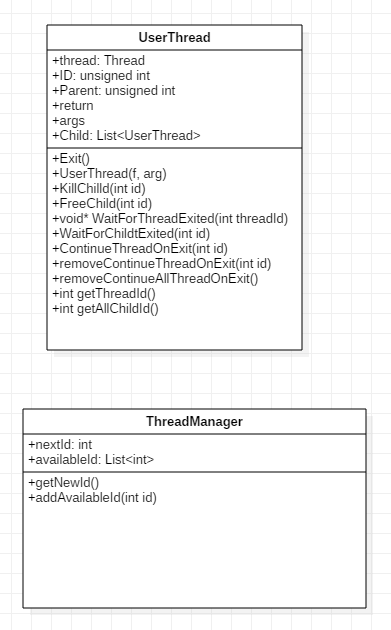
\includegraphics{code/userprog/UserThread.PNG}

Ainsi, chaque thread utilisateur sera associé à un thread kerbel grâce au stockage de l'adresse d'un UserThread dans la classe Thread du Kernel


Lorsqu'un appel système se déclenche, via le pointeur machine->currentThread ou se trouve un pointeur vers son UserThread, on pas alors utiliser les UserThread pour y appliquer les différentes opérations nécessaire.
\vspace{5mm}

L'assignation des identifiants d'UserThread se fait via le UserThreadManager. Le userThreadManager stock un variable compteur qui est incrémenter à chaque demande d'identifiant. C'est UserThread étant stocké sur des "unsigned int" on peux se voir limiter en nombre de thread parallèle par la limite de taille d'un unsigned int. Cependant, les identifiants sont recyclé. A chaque destruction de UserThread on réinjecter alors sont identifiant dans la liste du ThreadManager. Cela permet alors d'être sur qu'on programme à longue utilisation ne se retrouve jamais à cours d'identifiant. Néanmoins cela implique une plus grosse structure de stockage et une éventuelle perte temps par rapport à d'autre structure (exemple : bitmap)

\section{Scolaire}
\textit{une partie plus "scolaire" où vous décrivez l'organisation de votre travail (planning, ...), commentaires constructifs sur le déroulement du projet, ...}
\vspace{5mm}

\end{document}
